\documentclass[letterpaper]{scrreprt}
\usepackage{fourier}
\usepackage{amssymb,amsmath}
\usepackage{ifxetex,ifluatex}
\usepackage{fixltx2e} % provides \textsubscript
\ifnum 0\ifxetex 1\fi\ifluatex 1\fi=0 % if pdftex
  \usepackage[T1]{fontenc}
  \usepackage[utf8]{inputenc}
\else % if luatex or xelatex
  \ifxetex
    \usepackage{mathspec}
    \usepackage{xltxtra,xunicode}
  \else
    \usepackage{fontspec}
  \fi
  \defaultfontfeatures{Mapping=tex-text,Scale=MatchLowercase}
  \newcommand{\euro}{€}
\fi
% use upquote if available, for straight quotes in verbatim environments
\IfFileExists{upquote.sty}{\usepackage{upquote}}{}
% use microtype if available
\IfFileExists{microtype.sty}{%
\usepackage{microtype}
\UseMicrotypeSet[protrusion]{basicmath} % disable protrusion for tt fonts
}{}
\usepackage[margin=1in]{geometry}
\usepackage{graphicx}
\makeatletter
\def\maxwidth{\ifdim\Gin@nat@width>\linewidth\linewidth\else\Gin@nat@width\fi}
\def\maxheight{\ifdim\Gin@nat@height>\textheight\textheight\else\Gin@nat@height\fi}
\makeatother
% Scale images if necessary, so that they will not overflow the page
% margins by default, and it is still possible to overwrite the defaults
% using explicit options in \includegraphics[width, height, ...]{}
\setkeys{Gin}{width=\maxwidth,height=\maxheight,keepaspectratio}
\ifxetex
  \usepackage[setpagesize=false, % page size defined by xetex
              unicode=false, % unicode breaks when used with xetex
              xetex]{hyperref}
\else
  \usepackage[unicode=true]{hyperref}
\fi
\hypersetup{breaklinks=true,
            bookmarks=true,
            pdfauthor={Gus Dunn},
            pdftitle={Tsetse Collection Protocol},
            colorlinks=true,
            citecolor=blue,
            urlcolor=blue,
            linkcolor=magenta,
            pdfborder={0 0 0}}
\urlstyle{same}  % don't use monospace font for urls
\setlength{\parindent}{0pt}
\setlength{\parskip}{6pt plus 2pt minus 1pt}
\setlength{\emergencystretch}{3em}  % prevent overfull lines
\setcounter{secnumdepth}{5}

\title{Tsetse Collection Protocol\\\vspace{0.5em}{\large Core Procedures}}
\author{Gus Dunn}
\date{v0.2.1}

\begin{document}
\maketitle

{
\hypersetup{linkcolor=black}
\setcounter{tocdepth}{2}
\tableofcontents
}
\chapter{Deploying Traps}\label{deploying-traps}

\section{Materials}\label{materials}

\begin{itemize}
\itemsep1pt\parskip0pt\parsep0pt
\item
  Gum boots
\item
  GPS device
\item
  Panga
\item
  Mallet/hammer
\item
  Pencil(s)
\item
  razor (keeping pencil(s) sharp)
\item
  Paper for notes and trap-labels
\item
  Trap materials (see below)
\end{itemize}

\subsection{Per Trap}\label{per-trap}

\begin{itemize}
\itemsep1pt\parskip0pt\parsep0pt
\item
  1 metal rod (\textasciitilde{}2 meters long)
\item
  1 biconical fabric trap
\item
  1 collection cage and net sleeve
\item
  thick grease
\item
  \textasciitilde{}2 rubber bands
\end{itemize}

\section{Team}\label{team}

Deployment teams generally consist of 2 to 5 people. Gear is divided
among the team as works best but there are usually a few common classes
of roles.

\begin{description}
\item[Record Keeper]
carries the GPS device, a pencil, a pad of paper.
\item[Panga]
carries the panga and hammer.
\item[General Purpose]
carries what is needed. Some combination of trap materials as needed
including trap cones, collection cages/nets, grease, rubber bands.
\end{description}

\section{Procedures}\label{procedures}

\begin{itemize}
\itemsep1pt\parskip0pt\parsep0pt
\item
  As the team travels in the deployment area conducive sites are
  identified.
\item
  The \textbf{Record Keeper} places the date and trap number into the
  collection cage; records the trap's GPS coordinates \textbf{in DECIMAL
  DEGREES} format to 5 decimal places; and makes notes about the type of
  surrounding habitat as well as human activity in sight of the trap.
\item
  The site is cleared by the \textbf{Panga} and the rod is driven into
  the ground deep enough to provide robust ``staying power''.
\item
  The fabric cone is slipped onto the rod and the bottom is secured with
  a rubber band.
\item
  the tagged cage is added to the top and secured with a rubber band.
\item
  a \textbf{generous} amount of thick grease is applied to the rod below
  the cone such that the safari ants will be denied access to the trap
  cone and collection cage.
\end{itemize}

\begin{center}\rule{0.5\linewidth}{\linethickness}\end{center}

\chapter{Processing Flies}\label{processing-flies}

\section{Materials}\label{materials-1}

\emph{Not exhaustive, as specific needs may vary.}

\begin{itemize}
\itemsep1pt\parskip0pt\parsep0pt
\item
  Buffer for dissection etc
\item
  Microscope slides (with frosted labels)
\item
  Cover-slips
\item
  EtOH (100\%)
\item
  Cryo-tubes

  \begin{itemize}
  \itemsep1pt\parskip0pt\parsep0pt
  \item
    \textasciitilde{}2ml vol
  \item
    screw-top are best
  \end{itemize}
\item
  Specialized storage solution (if needed)
\item
  50ml `falcon' tubes for making personal solutions (washing forceps,
  etc)
\item
  Pasteur-type pipets
\item
  a couple p-1000 pippetmans
\item
  1 or more compound microscope (positive screening)
\item
  1 or more dissection scopes
\item
  gloves
\item
  permanent pens suitable for labeling the tubes
\item
  fine forceps for multiple stations
\item
  pencil(s)
\item
  razor (keeping pencil(s) sharp)
\item
  Parafilm M
\item
  tube racks / cryo-boxes
\item
  Kim-Wipes
\item
  Paper towels
\item
  Power generator and fuel (to run the scopes in the field if needed)
\item
  Voltage regulator/stabilizer
\item
  Field record data sheets
\item
  Adhesive labels for the sides of the cryo-tubes (Figure
  \ref{fig:labels})
\end{itemize}

\begin{figure}[htbp]
\centering

\includegraphics{figures/label_pad.jpg}
\caption{Labels typical of what is used at the \textbf{Label maker}
station. \label{fig:labels}}
\end{figure}

\section{Procedures}\label{procedures-1}

The fly processing is handled in an assembly-line format with stations
responsible for specific parts of the task (Figure \ref{fig:flow}).

\begin{figure}[htbp]
\centering
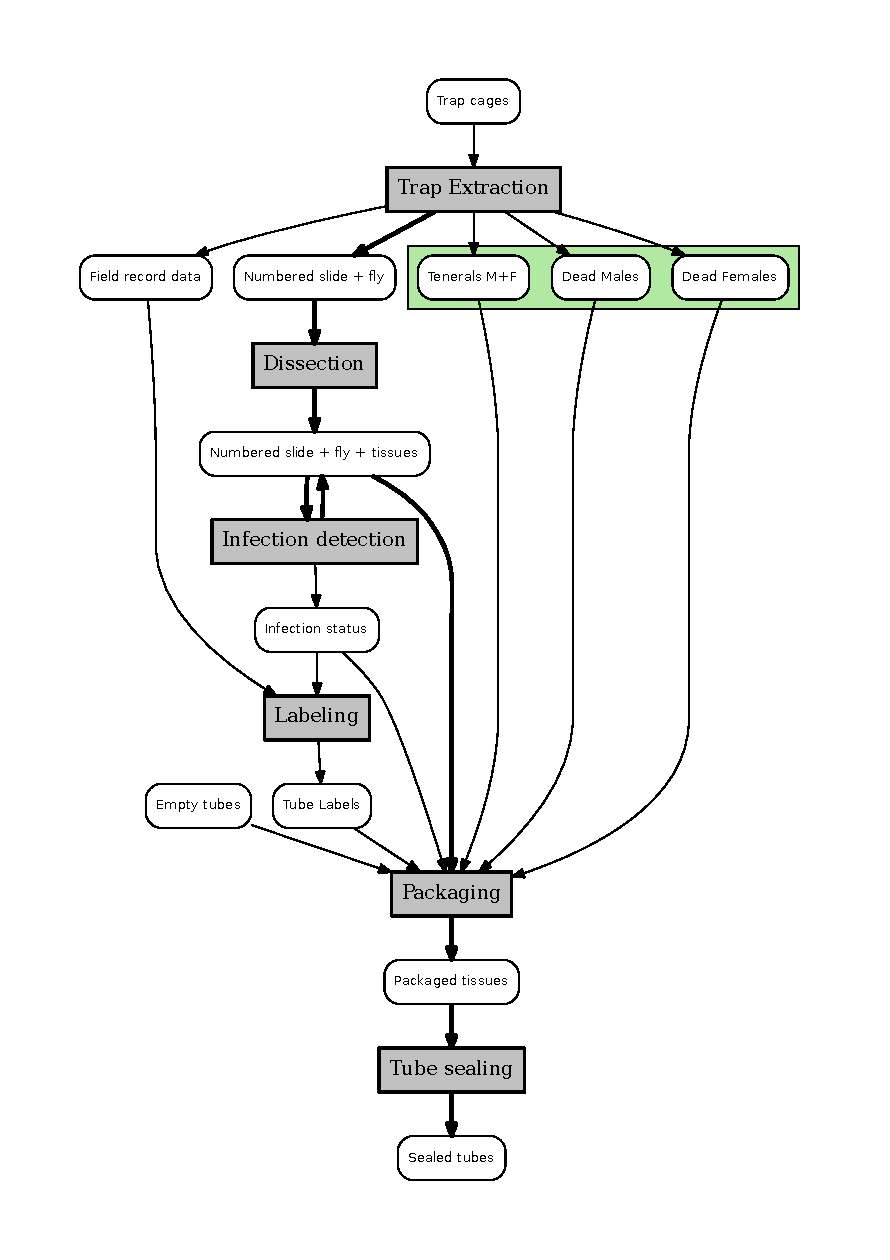
\includegraphics{figures/fly_processing_flow.pdf}
\caption{Basic Processing Flow -- Grey boxes are processing stations.
White rounded boxes are inputs/outputs of processing stations. Arrows
show the flow of processing materials. BOLD arrows show the flow of fly
materials. The green box represents materials set aside for processing
after the live flies have been processed. \label{fig:flow}}
\end{figure}

\subsection{Trap extraction station}\label{trap-extraction-station}

This station is responsible for removing the flies from the cage of the
current trap and recording the initial information for this fly in the
field collection sheet\footnote{To obtain the sheets that we used in the
  field you will need to contact Richard Echodu
  (richardechodu2009@gmail.com), but the excel file templates we sent
  should give an idea of what is included.}. This information includes
(but may not be limited to):

\begin{itemize}
\itemsep1pt\parskip0pt\parsep0pt
\item
  date (once per sheet)
\item
  trap number
\item
  the fly number
\item
  sex
\item
  hunger stage and/or wing fray
\item
  collection date
\item
  town name/ID symbol
\end{itemize}

\emph{For each fly:}

\begin{enumerate}
\def\labelenumi{\arabic{enumi}.}
\itemsep1pt\parskip0pt\parsep0pt
\item
  Incapacitate fly by cracking its head or some other way of killing the
  fly without causing too much physical destruction to the fly.
\item
  Collect and record in the field record sheet the prescribed
  information (see above list).
\item
  Place fly on microscope slide with a frosted labeling end.
\item
  Write the number that corresponds to this fly in the field record
  sheet on the slide label with \emph{pencil}.
\item
  Send slide to \textbf{Dissection}.
\end{enumerate}

\emph{Remarks:}

\begin{itemize}
\itemsep1pt\parskip0pt\parsep0pt
\item
  \textbf{Don't get bitten}.
\item
  \textbf{Close attention} must be paid to ensure the number on the
  slide matches the number for each fly in the field record. If
  \emph{even \textbf{ONE}} numbered fly is mistakenly left out of the
  processing stream or an additional added to the stream it will cause
  \textbf{ALL SUBSEQUENT fly information} to be incorrect\footnote{Similar
    to a frame-shift mutation: it shifts the register of identities out
    of sync with all remaining flies.}.
\end{itemize}

\subsection{Labeling station}\label{labeling-station}

\begin{itemize}
\item
  This station does not strictly ``follow'' in the assembly-line but is
  more of a concurrent station with the \textbf{Trap extraction}
  station.
\item
  The \textbf{Labeling} station writes the relevant information for each
  fly as it is being removed from the trap and incapacitated in
  preparation for dissection.
\item
  The information is recorded in pencil on a pad of small labels that
  will be placed on each tube (by the \textbf{Packaging} station) that
  contains part of the fly with the corresponding number (Figure
  \ref{fig:labels}).
\item
  The important information to be recorded is:

  \begin{itemize}
  \itemsep1pt\parskip0pt\parsep0pt
  \item
    Location code
  \item
    Date (\texttt{MM-DD})
  \item
    Fly number
  \item
    Trap number
  \item
    Tissue code (Something like: M, S, C, H \textasciitilde{} Midgut,
    Salivary glands, Carcass, Head)
  \end{itemize}
\item
  A label must be written for each tube that a fly will be packed into.

  \begin{itemize}
  \itemsep1pt\parskip0pt\parsep0pt
  \item
    If you are collecting carcass and midguts: two labels with the above
    information will be generated for each fly and given to
    \textbf{Packaging}.
  \end{itemize}
\item
  Periodically, the labels are sent to the \textbf{Packaging} station(s)
  for application to the tubes.
\end{itemize}

\emph{Remarks:}

\begin{itemize}
\itemsep1pt\parskip0pt\parsep0pt
\item
  The sooner that \textbf{Packaging} gets these labels, the faster the
  whole process will go and the less likely it will be that flies become
  mislabeled.
\end{itemize}

\subsection{Dissection station}\label{dissection-station}

\emph{For each fly:}

\begin{enumerate}
\def\labelenumi{\arabic{enumi}.}
\itemsep1pt\parskip0pt\parsep0pt
\item
  \textbf{Wash tools (forceps/scissors/etc) in 90\% EtOH and wipe with
  Kim-Wipes to avoid contamination of current fly.}
\item
  Dissect according to the needs of the collection trip.
\item
  Organize tissues on the slide in PBS so as to best facilitate the
  inspection for positives in next station.
\item
  Send slide to \textbf{Infection status}.
\end{enumerate}

\emph{Remarks:}

\begin{itemize}
\itemsep1pt\parskip0pt\parsep0pt
\item
  Avoid cross contaminating flies with Trypanosomes by frequent and
  thorough cleaning of your forceps etc.
\end{itemize}

\subsection{Infection detection
station}\label{infection-detection-station}

\emph{For each fly:}

\begin{enumerate}
\def\labelenumi{\arabic{enumi}.}
\itemsep1pt\parskip0pt\parsep0pt
\item
  \textbf{Wash tools (forceps/scissors/etc) in 90\% EtOH and wipe with
  Kim-Wipes to avoid contamination of current fly.}
\item
  Examine tissues for signs of Trypanosome infection.
\item
  Call out the infection status for \textbf{Labeling} and
  \textbf{Packaging}.

  \begin{itemize}
  \itemsep1pt\parskip0pt\parsep0pt
  \item
    in practice calling out only the status of flies that are positive
    is sufficient.
  \item
    if you are able to distinguish between low, medium, and high levels
    of infection, it is good to do so.
  \end{itemize}
\item
  Pass slide to \textbf{Packaging}.
\end{enumerate}

\emph{Remarks:}

\begin{itemize}
\itemsep1pt\parskip0pt\parsep0pt
\item
  Avoid cross contaminating flies with Trypanosomes by frequent and
  thorough cleaning of your forceps etc.
\end{itemize}

\subsection{Packaging station}\label{packaging-station}

\emph{For each fly:}

\begin{enumerate}
\def\labelenumi{\arabic{enumi}.}
\itemsep1pt\parskip0pt\parsep0pt
\item
  \textbf{Wash tools (forceps/scissors/etc) in 90\% EtOH and wipe with
  Kim-Wipes to avoid contamination of current fly.}
\item
  Assemble enough tubes (\emph{pre-filled with \textasciitilde{}250ul of
  90\% EtOH or appropriate storage solution}) to receive the number of
  separate tissues dictated by the needs of this collection.
\item
  If possible, use the labels generated by \textbf{Labeling} to
  pre-label the tubes to reduce confusion.
\item
  Package the tissues in correctly labeled tubes as swiftly as possible
  \emph{while maintaining control of quality}.
\item
  \textbf{Double-check} that each tube has the correct side-label, then
  label the tube top with \emph{only} the Site-ID code and fly number
  using lab marker/sharpie.
\item
  If the fly has a positive status, add a code to the side-label:

  \begin{itemize}
  \itemsep1pt\parskip0pt\parsep0pt
  \item
    \texttt{\textquotesingle{}+\textquotesingle{}} = low to normal
    infection level
  \item
    \texttt{\textquotesingle{}++\textquotesingle{}} = mid to high
    infection
  \item
    \texttt{\textquotesingle{}+++\textquotesingle{}} = very high
    infection
  \end{itemize}
\end{enumerate}

\emph{After the live flies have been processed:}

\begin{enumerate}
\def\labelenumi{\arabic{enumi}.}
\itemsep1pt\parskip0pt\parsep0pt
\item
  All teneral\footnote{An adult too young to have bloodfed.} flies: live
  or dead are placed into communal falcon tubes by Village (or
  approximately synonymous site level).

  \begin{itemize}
  \itemsep1pt\parskip0pt\parsep0pt
  \item
    males and females can be combined
  \end{itemize}
\item
  Dead non-teneral flies are separated by sex and placed into communal
  falcon tubes by Village.
\item
  Communal tubes are labeled with information analogous to individual
  flies except that there is no fly number and the number of flies
  contained in each falcon tube is included.
\item
  Add enough 90\% EtOH to cover the flies sufficiently, allowing for
  some extra.
\item
  This information should match the info recorded in the field data
  sheets.
\end{enumerate}

\emph{Remarks:}

\begin{itemize}
\itemsep1pt\parskip0pt\parsep0pt
\item
  Avoid cross contaminating flies with Trypanosomes by frequent and
  thorough cleaning of your forceps etc.
\item
  Pre-filling hundreds of tubes with \textasciitilde{}250ul of EtOH the
  night before will save you \textbf{enormous} time and pain during the
  processing sessions and reduce the likelihood of mistakes.
\end{itemize}

\subsection{Tube sealing station}\label{tube-sealing-station}

\begin{enumerate}
\def\labelenumi{\arabic{enumi}.}
\itemsep1pt\parskip0pt\parsep0pt
\item
  Get a strip of parafilm with dimensions approximately 2 inches
  long/\textasciitilde{}0.5 inches wide (\textasciitilde{}5cm Long
  /\textasciitilde{}1.5cm Wide).
\item
  Stretch it about 1.5 times around the tube where the label is affixed.
\item
  Break it off.
\item
  Stretch the rest around the seam where the top meets the tube: make
  sure that it covers the writing on the tube top AND seals the seam.
\item
  Organize the tubes in boxes or bags with a system similar to the
  following:

  \begin{itemize}
  \itemsep1pt\parskip0pt\parsep0pt
  \item
    tubes of the same tissue type are stored together with other tubes
    with the same site-code (\textasciitilde{}Village level)
  \item
    Bags/boxes above can be placed into larger bags that group a
    particular \textasciitilde{}village etc.
  \end{itemize}
\end{enumerate}

\emph{Remarks:}

\begin{itemize}
\itemsep1pt\parskip0pt\parsep0pt
\item
  \emph{Use this opportunity to double-check that the side-labels of
  each tube match the tube-tops.}
\item
  This step is best done \textbf{by everyone} following the completion
  of the main processing queue.
\item
  Doing this on the same day as the processing of the tubes is best.
\item
  If the tubes are to be transported by plane/bus/over-seas, the quality
  of this step may be considered directly proportional to the ability of
  the tubes to be used correctly in the lab and therefore to the quality
  of results possible.
\end{itemize}

\begin{center}\rule{0.5\linewidth}{\linethickness}\end{center}

\chapter{Milking Traps}\label{milking-traps}

\section{Materials}\label{materials-2}

\begin{itemize}
\itemsep1pt\parskip0pt\parsep0pt
\item
  See materials list for Trap Deploying.
\end{itemize}

\section{Procedures}\label{procedures-2}

\begin{itemize}
\itemsep1pt\parskip0pt\parsep0pt
\item
  The teams may be 2-3 people.
\item
  Multiple teams per location may operate simultaneously to speed
  recovery of trap cages.
\item
  Each team should have pencil and paper to place a labeled piece of
  paper\footnote{Should contain the new date and same trap number.} in
  the new trap cage that they use to replace the retrieved trap cage for
  each trap.
\item
  Retrieved trap cages should be handled in such a way to reduce the
  death rate before processing can be begun.

  \begin{itemize}
  \itemsep1pt\parskip0pt\parsep0pt
  \item
    shade
  \item
    avoid excessive temps
  \item
    out of access from ants etc.
  \end{itemize}
\end{itemize}

\begin{center}\rule{0.5\linewidth}{\linethickness}\end{center}

\chapter{Recovering Traps}\label{recovering-traps}

\section{Materials}\label{materials-3}

\begin{itemize}
\itemsep1pt\parskip0pt\parsep0pt
\item
  See materials list for Trap Deploying.
\end{itemize}

\section{Procedures}\label{procedures-3}

\begin{itemize}
\itemsep1pt\parskip0pt\parsep0pt
\item
  Teams may be smaller for trap recovery.
\item
  Multiple teams per location may operate simultaneously to speed
  recovery of traps.
\item
  Traps are disassembled and cages retrieved if flies are to be
  collected.
\item
  Rods are cleaned on the grass etc to remove the grease.
\end{itemize}

\begin{center}\rule{0.5\linewidth}{\linethickness}\end{center}

\chapter{Appendices}\label{appendices}

\section{Collection Documentation
Files}\label{collection-documentation-files}

\subsection{Collection Data
Spreadsheet}\label{collection-data-spreadsheet}

\subsubsection{Purpose:}\label{purpose}

\begin{itemize}
\itemsep1pt\parskip0pt\parsep0pt
\item
  Provides an electronic version of the data recorded for each
  \textbf{fly} during the field collection efforts.
\item
  Allows data to easily shared with collaborators.
\item
  Allows data to be imported into computer-based sample tracking
  database in an automated fashion.
\end{itemize}

\subsubsection{Column descriptions:}\label{column-descriptions}

Below are the definitions for the type and format of data recorded in
each column of this file type. Fields denoted with an asterisk are
required if the data exist. The rest are technically optional but are
still \emph{very} important to include if you have the information.

\begin{enumerate}
\def\labelenumi{\Alph{enumi}.}
\itemsep1pt\parskip0pt\parsep0pt
\item
  \textbf{Village*:}

  \begin{itemize}
  \itemsep1pt\parskip0pt\parsep0pt
  \item
    Please list an appropriate name for the location common to a set of
    traps. This should be a village name or something at a similar level
    of resolution.
  \end{itemize}
\item
  \textbf{Trap\_No*:}

  \begin{itemize}
  \itemsep1pt\parskip0pt\parsep0pt
  \item
    A number or other ID specific to a single trap.
  \end{itemize}
\item
  \textbf{Date*:}

  \begin{itemize}
  \itemsep1pt\parskip0pt\parsep0pt
  \item
    The date these flies were collected from the trap.
  \item
    The date should be formatted as \texttt{YYYY-MM-DD} to avoid
    ambiguity and ensure correct computer sorting.
  \end{itemize}
\item
  \textbf{Species*:}

  \begin{itemize}
  \itemsep1pt\parskip0pt\parsep0pt
  \item
    Use either the full species name of the fly or the first letter of
    each word. Examples: \emph{Glossina fuscipes fuscipes} or Gff.
  \end{itemize}
\item
  \textbf{Sex*:}

  \begin{itemize}
  \itemsep1pt\parskip0pt\parsep0pt
  \item
    Use the letter \textbf{M} or \textbf{F} for male or female,
    respectively.
  \end{itemize}
\item
  \textbf{Teneral*:}

  \begin{itemize}
  \itemsep1pt\parskip0pt\parsep0pt
  \item
    Use the codes \textbf{T} or \textbf{NT} for teneral or non-teneral,
    respectively.
  \end{itemize}
\item
  \textbf{Dead*:}

  \begin{itemize}
  \itemsep1pt\parskip0pt\parsep0pt
  \item
    Use the letter \textbf{D} or \textbf{L} if the fly was dead or
    alive, respectively, at the time that the trap contents were being
    processed.
  \end{itemize}
\item
  \textbf{Fly\_Number*:}

  \begin{itemize}
  \itemsep1pt\parskip0pt\parsep0pt
  \item
    A unique number assigned to each fly collected during a collection
    trip.
  \end{itemize}
\item
  \textbf{Hunger\_stage:}

  \begin{itemize}
  \item
    Hunger stage as defined in:

    \begin{enumerate}
    \def\labelenumii{\arabic{enumii}.}
    \itemsep1pt\parskip0pt\parsep0pt
    \item
      Jackson, C. H. N. The Causes and Implications of Hunger in
      Tsetse-flies. Bull. Entomol. Res. 24, 443--482 (1933).
    \item
      Leak, S. G. A. Tsetse biology and ecology: their role in the
      epidemiology and control of trypanosomosis. (ILRI (aka ILCA and
      ILRAD), 1999).
    \end{enumerate}
  \item
    Value range: 1 to 4
  \item
    If not collected: enter ``NA''.
  \end{itemize}
\item
  \textbf{Wing\_fray:}

  \begin{itemize}
  \itemsep1pt\parskip0pt\parsep0pt
  \item
    If this measure is appropriate and you normally record it, you can
    place it here; if not, enter ``NA''.
  \end{itemize}
\item
  \textbf{prob:}

  \begin{itemize}
  \itemsep1pt\parskip0pt\parsep0pt
  \item
    If this tissue (proboscis) was checked for trypanosome infection,
    enter ``0'' for negative and ``1'' for positive results, ``NA''
    otherwise.
  \end{itemize}
\item
  \textbf{midgut:}

  \begin{itemize}
  \itemsep1pt\parskip0pt\parsep0pt
  \item
    If this tissue (midgut) was checked for trypanosome infection, enter
    ``0'' for negative and ``1'' for positive results, ``NA'' otherwise.
  \end{itemize}
\item
  \textbf{sal\_gland:}

  \begin{itemize}
  \itemsep1pt\parskip0pt\parsep0pt
  \item
    If this tissue (salivay gland) was checked for trypanosome
    infection, enter ``0'' for negative and ``1'' for positive results,
    ``NA'' otherwise.
  \end{itemize}
\item
  \textbf{Kept\_in:}

  \begin{itemize}
  \itemsep1pt\parskip0pt\parsep0pt
  \item
    Please list the solution that the sample is stored in.
  \end{itemize}
\item
  \textbf{Comment:}

  \begin{itemize}
  \itemsep1pt\parskip0pt\parsep0pt
  \item
    Any comments that you think should be recorded about this sample.
  \end{itemize}
\item
  \textbf{Tube\_or\_box:}

  \begin{itemize}
  \itemsep1pt\parskip0pt\parsep0pt
  \item
    Is this a box of existing samples of DNA or other extracted
    materials? Then choose ``box''. Otherwise, choose ``tube''.
  \end{itemize}
\item
  \textbf{Tissue:}

  \begin{itemize}
  \item
    When the sample is a material like DNA that has been derived from a
    part of or a whole fly, please list the tissue that was used to
    extract the DNA. A list of common tissues has been provided for your
    convenience, but non-listed values are allowed.

    \begin{itemize}
    \itemsep1pt\parskip0pt\parsep0pt
    \item
      carcass
    \item
      head
    \item
      antennae
    \item
      midgut
    \item
      proventriculus
    \item
      midgut + proventriculus
    \item
      salivary glands
    \item
      reproductive parts
    \item
      legs
    \item
      whole
    \end{itemize}
  \end{itemize}
\item
  \textbf{Method\_of\_prep:}

  \begin{itemize}
  \itemsep1pt\parskip0pt\parsep0pt
  \item
    If the sample is DNA or another derived material, please include a
    brief comment about what method/kit was used to generate the
    material.
  \end{itemize}
\end{enumerate}

\subsection{Collection Summary
Spreadsheet}\label{collection-summary-spreadsheet}

\subsubsection{Purpose:}\label{purpose-1}

\begin{itemize}
\itemsep1pt\parskip0pt\parsep0pt
\item
  Provides an electronic version of the data recorded for each
  \textbf{trap} during the field collection efforts.
\item
  Allows data to easily shared with collaborators.
\item
  Allows data to be imported into computer-based sample tracking
  database in an automated fashion.
\end{itemize}

\subsubsection{Column descriptions:}\label{column-descriptions-1}

Below are the definitions for the type and format of data recorded in
each column of this file type. Fields denoted with an asterisk are
required if the data exist. The rest are technically optional but are
still \emph{very} important to include if you have the information.

\begin{enumerate}
\def\labelenumi{\Alph{enumi}.}
\itemsep1pt\parskip0pt\parsep0pt
\item
  \textbf{District:}

  \begin{itemize}
  \itemsep1pt\parskip0pt\parsep0pt
  \item
    District or similar level of administrative hierarchy.
  \end{itemize}
\item
  \textbf{County:}

  \begin{itemize}
  \itemsep1pt\parskip0pt\parsep0pt
  \item
    County or similar level of administrative hierarchy.
  \end{itemize}
\item
  \textbf{Subcounty:}

  \begin{itemize}
  \itemsep1pt\parskip0pt\parsep0pt
  \item
    Subcounty or similar level of administrative hierarchy.
  \end{itemize}
\item
  \textbf{Parish:}

  \begin{itemize}
  \itemsep1pt\parskip0pt\parsep0pt
  \item
    Parish or similar level of administrative hierarchy.
  \end{itemize}
\item
  \textbf{Village*:}

  \begin{itemize}
  \itemsep1pt\parskip0pt\parsep0pt
  \item
    Village or similar level of administrative hierarchy.
  \end{itemize}
\item
  \textbf{Trap\_No*:}

  \begin{itemize}
  \itemsep1pt\parskip0pt\parsep0pt
  \item
    A number or other ID specific to a single trap.
  \end{itemize}
\item
  \textbf{Latitude*:}

  \begin{itemize}
  \itemsep1pt\parskip0pt\parsep0pt
  \item
    Latitude GPS coordinates for the trap \textbf{in DECIMAL DEGREES}
    format to 5 decimal places.
  \end{itemize}
\item
  \textbf{Longitude*:}

  \begin{itemize}
  \itemsep1pt\parskip0pt\parsep0pt
  \item
    Longitude GPS coordinates for the trap \textbf{in DECIMAL DEGREES}
    format to 5 decimal places.
  \end{itemize}
\item
  \textbf{Elevation\_in\_m*:}

  \begin{itemize}
  \itemsep1pt\parskip0pt\parsep0pt
  \item
    Elevation at the trap's location in meters (m).
  \end{itemize}
\item
  \textbf{Human\_Activity:}

  \begin{itemize}
  \itemsep1pt\parskip0pt\parsep0pt
  \item
    A short (10 words or less if possible) description of the type of
    human activity within sight of the trap's location.
  \item
    farm plots, livestock, home, road, etc.
  \end{itemize}
\item
  \textbf{Vegtype:}

  \begin{itemize}
  \itemsep1pt\parskip0pt\parsep0pt
  \item
    A short classification of the type of vegetation around the trap
    location.
  \item
    riverine, savannah, etc.
  \end{itemize}
\item
  \textbf{Deploy\_date*:}

  \begin{itemize}
  \itemsep1pt\parskip0pt\parsep0pt
  \item
    The date this trap was deployed.
  \item
    The date should be formatted as \texttt{YYYY-MM-DD} to avoid
    ambiguity and ensure correct computer sorting.
  \end{itemize}
\item
  \textbf{Harvest\_date*:}

  \begin{itemize}
  \itemsep1pt\parskip0pt\parsep0pt
  \item
    The date this trap was removed.
  \item
    The date should be formatted as \texttt{YYYY-MM-DD} to avoid
    ambiguity and ensure correct computer sorting.
  \end{itemize}
\item
  \textbf{Male*:}

  \begin{itemize}
  \itemsep1pt\parskip0pt\parsep0pt
  \item
    the number of males collected from this trap.
  \end{itemize}
\item
  \textbf{Female*:}

  \begin{itemize}
  \itemsep1pt\parskip0pt\parsep0pt
  \item
    the number of feales collected from this trap.
  \end{itemize}
\item
  \textbf{Total*:}

  \begin{itemize}
  \itemsep1pt\parskip0pt\parsep0pt
  \item
    the number of flies total collected from this trap.
  \end{itemize}
\item
  \textbf{FTD:}

  \begin{itemize}
  \itemsep1pt\parskip0pt\parsep0pt
  \item
    (\textbf{F})lies per (\textbf{T})rap per (\textbf{D})ay
  \item
    Mean number of flies caught in this trap per day.
  \item
    Divide `\textbf{Total}' number by the number of days the trap was
    deployed.
  \end{itemize}
\item
  \textbf{Other\_info:}

  \begin{itemize}
  \itemsep1pt\parskip0pt\parsep0pt
  \item
    Other information pertaining to a trap that you feel would be
    useful.
  \end{itemize}
\end{enumerate}

\end{document}
